\chapter{building tempest 2000 in 1994}
\label{sec:building_t2k}
\lstset{style=68KStyle}
\lhead[tempest 2000]{}

It is 1994 and Atari have asked you create the flagship launch title for their new video game console,
the Atari Jaguar. No need to come to Sunnyvale in California, you can stay in your valley in Wales and
let us know when you're finished.

\begin{figure}[H]
      \centering
      \frame{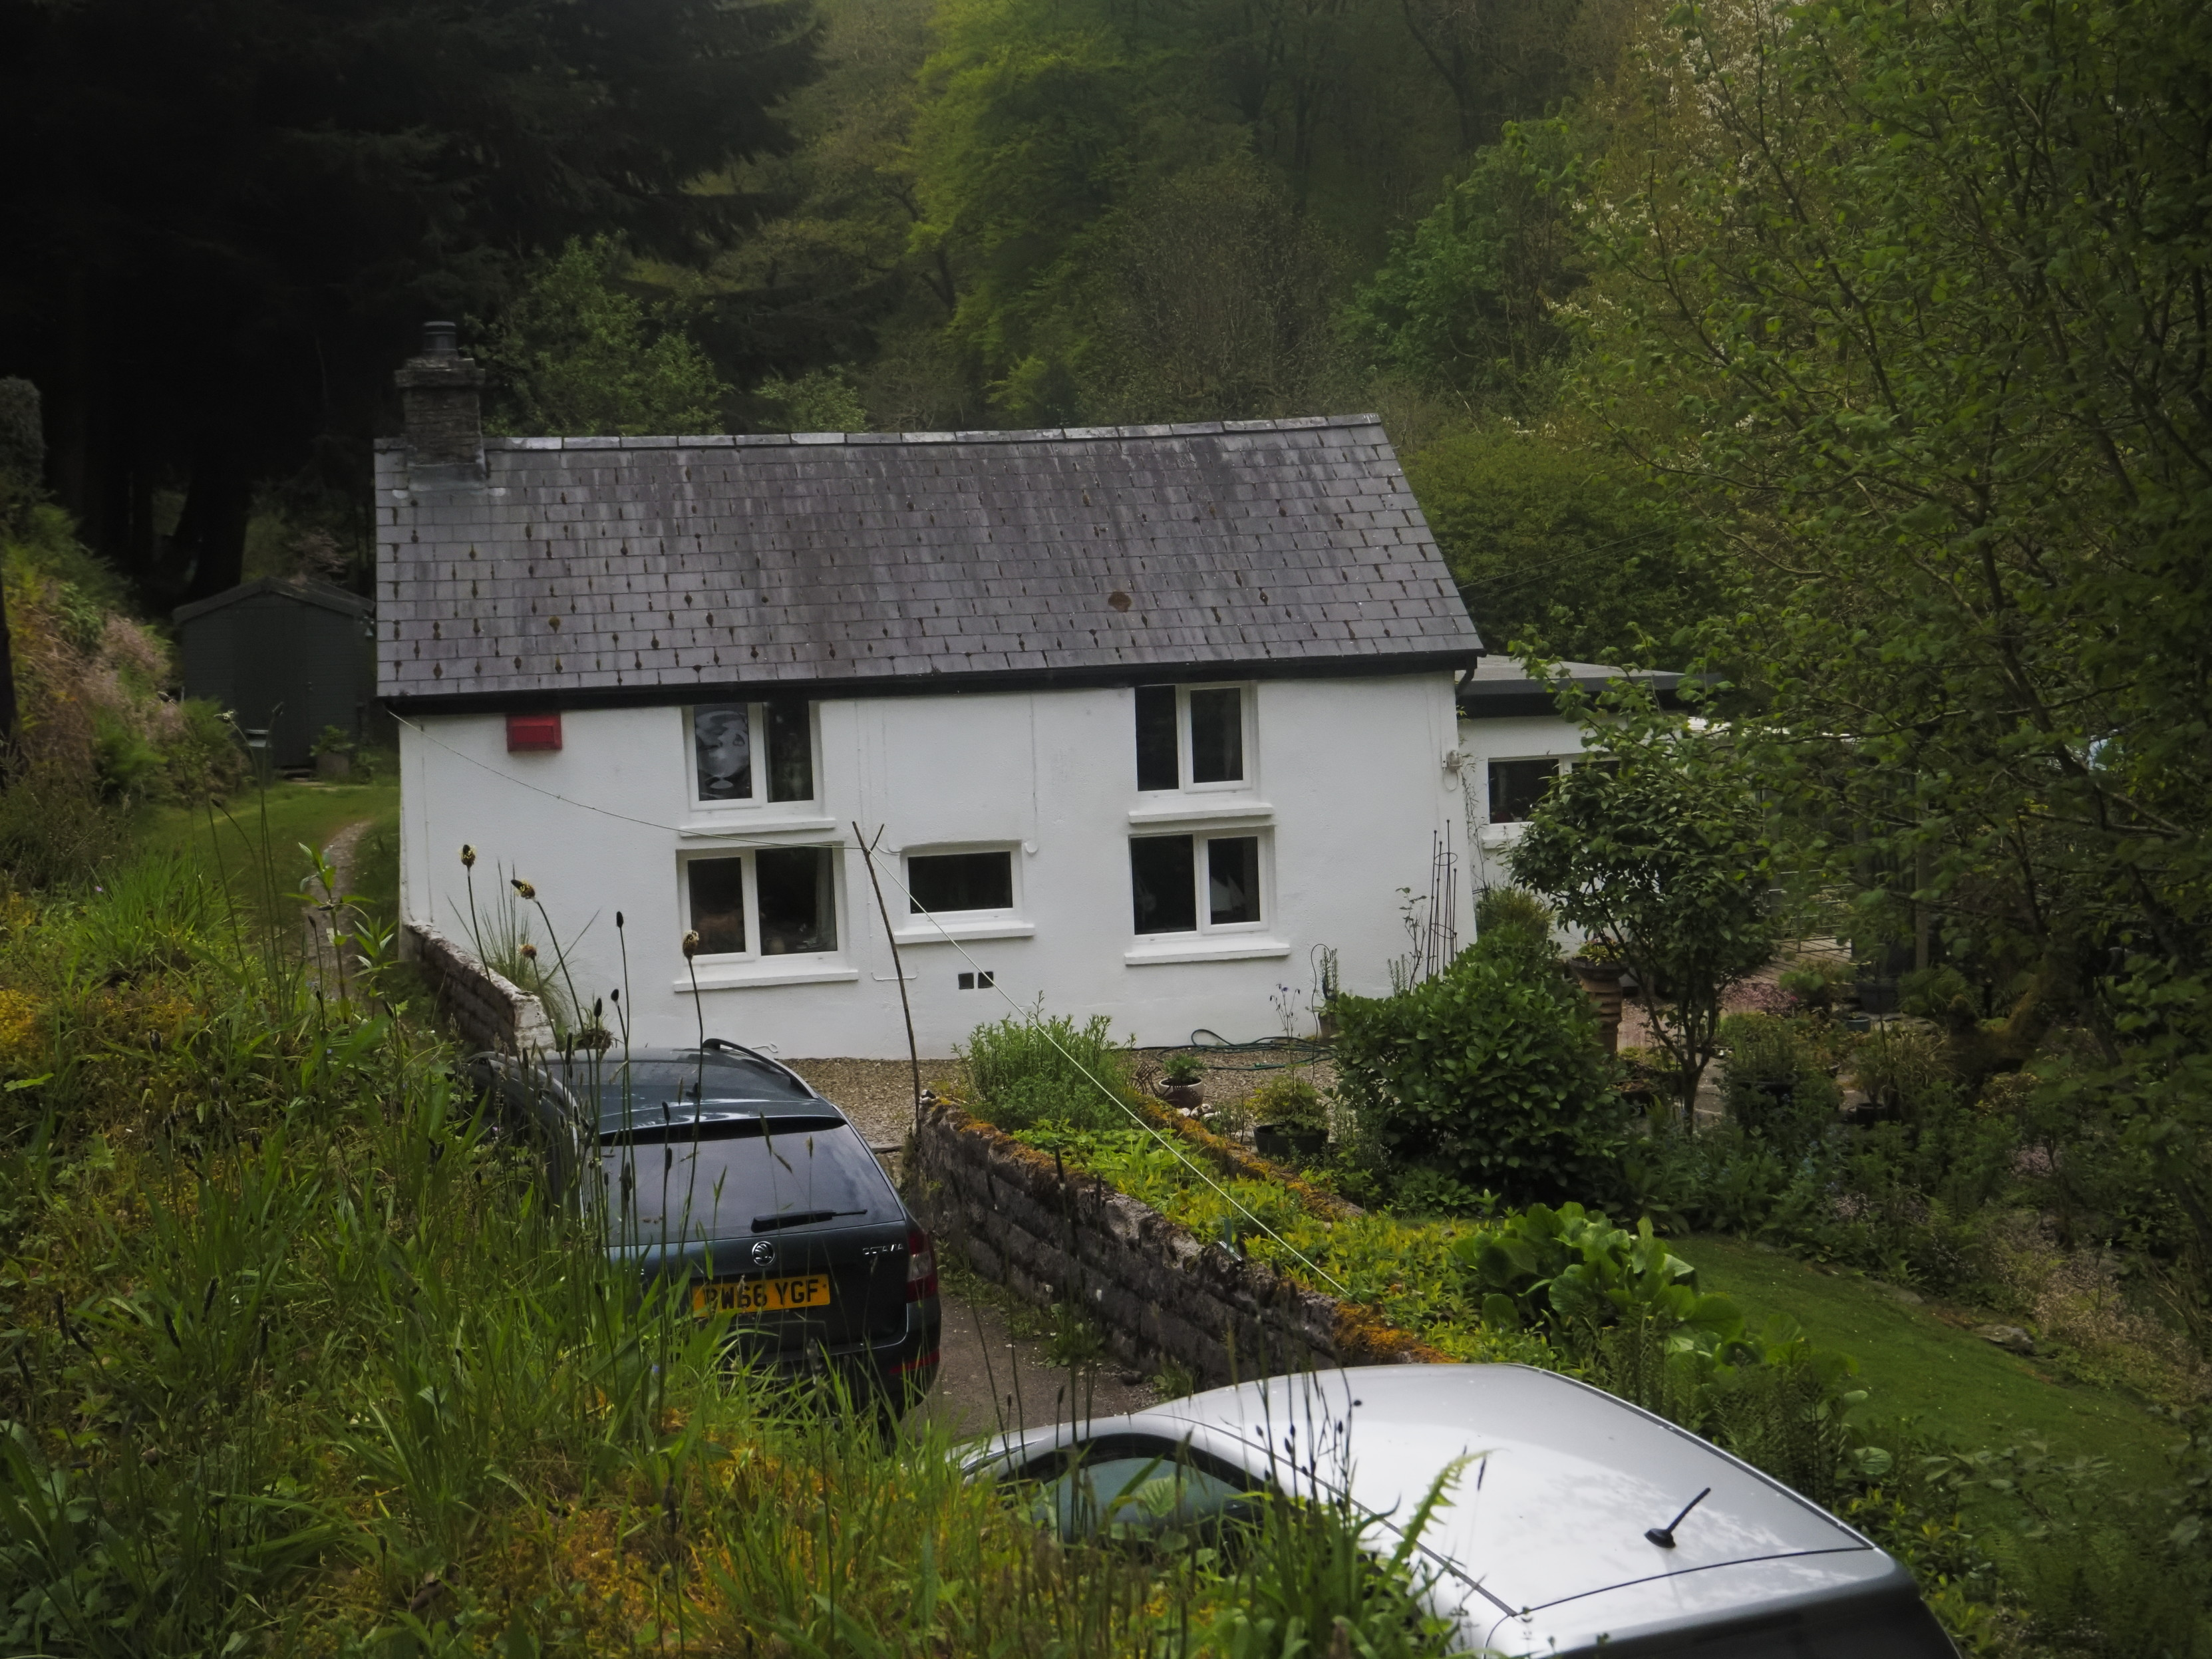
\includegraphics[width=8cm]{src/build_t2k/cwmcych.jpg}}%
    \caption{You are not in California, you are in Cwmcych in Wales and that's where you'll make Tempest 2000.}
\end{figure}

So instead of sitting two doors down from the computer room armed with just a pencil, you are instead 
expected to conjure a game that will launch a machine on which the future of Atari depends from your cottage.
To get you started you will be sent a console and a manual. You already have a computer we assume.

So because it's the way you've always done it, you get started writing \icode{Tempest 2000} in one big file
of Motoral 68K assembly code.
And because you always get to name things whatever you want, you name this file \icode{YAK.S}, because that's the 
the three-letter name you use on high score tables.

\begin{figure}[H]
      \centering
      \frame{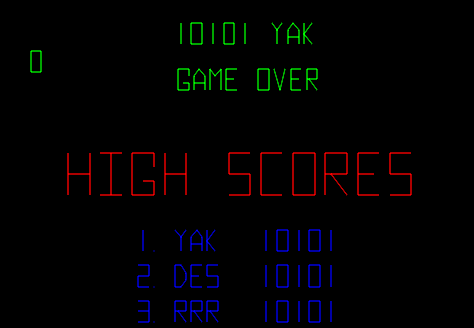
\includegraphics[width=8cm]{src/build_t2k/yak.png}}%
    \caption{YAK has the top score in Tempest.}
\end{figure}

Assembling this code will be 
